% Chapter Template

\externaldocument{Chapter2}

\chapter{Podstawowe algorytmy stabilizacji lotu kwadrokopterów} % Main chapter title

\label{Chapter3} % Change X to a consecutive number; for referencing this chapter elsewhere, use \ref{ChapterX}

\lhead{Rozdział 3. \emph{Podstawowe algorytmy stabilizacji lotu kwadrokopterów}} % Change X to a consecutive number; this is for the header on each page - perhaps a shortened title

%----------------------------------------------------------------------------------------
%	SECTION 1
%----------------------------------------------------------------------------------------

\section{Podstawy matematyczne}

Fizyczne podstawy lotu opisane w rozdziale~\ref{Chapter2} tłumaczą, że ruch postępowy kwadrokoptera w pionie jest wynikiem braku równowagi między wypadkową siłą ciągu wszystkich silników a siłą grawitacji działającą na urządzenie, natomiast ruch w płaszczyźnie poziomej dla konfiguracji przedstawionej na rysunku ~\ref{fig:quadrotor_forces} jest wynikiem obrotu kwadrokoptera wokół osi $X_b$ lub $Y_b$~\cite{quadro8, quadro9}. Wiadomo również, że wypadkowa siła działająca na kwadrokopter może być zmieniana poprzez proporcjonalną zmianę prędkości obrotowych wszystkich czterech wirników jednocześnie, oraz że obrót kwadrokoptera wokół dowolnej jego osi jest wynikiem braku równowagi między prędkościami kątowymi odpowiednich par wirników. Informacje te prowadzą do konkluzji, że wszystkie sześć stopni swobody kwadrokoptera może być kontrolowanych jedynie za pomocą odpowiedniej zmiany prędkości obrotowych wirników. Powstaje zatem pytanie, w jaki sposób kontrolować prędkości obrotowe wirników, chcąc uzyskać zamierzoną zmianę położenia kwadrokoptera w przestrzeni. 

Rozważmy model kwadrokoptera przedstawiony na rysunku ~\ref{fig:quadrotor_forces}. Dla tak oznaczonych osi oraz numeracji silników możemy zapisać następujący komplet równań~\cite{quadro9}:
\begin{equation}
\begin{aligned}
	\dot{\phi} &= k_r((\omega_1 + \omega_4) - (\omega_2 + \omega_3)) \\
	\dot{\theta} &= k_p((\omega_1 + \omega_2) - (\omega_3 + \omega_4)) \\
	\dot{\psi} &= k_y((\omega_1 + \omega_3) - (\omega_2 + \omega_4)) \\
	f &= k_t(\omega_1 + \omega_2 + \omega_3 + \omega_4)
\end{aligned}
\end{equation}

gdzie $\dot{\phi}$, $\dot{\theta}$, $\dot{\psi}$ są prędkościami kątowymi odpowiednio wokół osi $X_b$, $Y_b$, $Z_b$, wypadkowa siła ciągu silników została oznaczona jako $f$, a $k_r$, $k_p$, $k_y$, $k_t$ są współczynnikami proporcjonalności zależnymi od własności fizycznych systemu. Po opuszczeniu nawiasów i uszeregownaiu zmiennych, powyższy układ równań nabiera następującej postaci:

\begin{equation}
\begin{aligned}
	\dot{\phi} &= k_r\omega_1 - k_r\omega_2 - k_r\omega_3 + k_r\omega_4 \\
	\dot{\theta} &= k_p\omega_1 + k_p\omega_2 - k_p\omega_3 - k_p\omega_4 \\
	\dot{\psi} &= k_y\omega_1 - k_y\omega_2 + k_y\omega_3 - k_y\omega_4 \\
	f &= k_t\omega_1 + k_t\omega_2 + k_t\omega_3 + k_t\omega_4
\end{aligned}
\end{equation}



Przyjmując w uproszczeniu, że $k_r = k_p = k_y = k_t = k$, możemy zapisać powyższy komplet równań w postaci macierzowej:

\begin{equation}
	\label{eq:omega_as_argument}
	\begin{pmatrix}
		\dot{\phi} \\
		\dot{\theta} \\
		\dot{\psi} \\
		f
	\end{pmatrix} = 
	\begin{pmatrix}
		k & -k & -k & k \\
		k & k & -k & -k \\
		k & -k & k & -k \\
		k & k & k & k
	\end{pmatrix}
	\begin{pmatrix}
		\omega_1 \\
		\omega_2 \\
		\omega_3 \\
		\omega_4
	\end{pmatrix}
\end{equation}

Jak widać, powyższy zestaw równań odpowiada na pytanie, w jaki sposób prędkości obrotowe kwadrokoptera wokół osi układu współrzędnych, oraz wypadkowa siła zależą od prędkości obrotowych wirników. Chcąc kontrolować położenie i orientację kwadrokoptera w przestrzeni musimy wyrazić prędkości obrotowe śmigieł jako funkcję zadanych prędkości obrotowych kwadrokoptera wokół osi układu odniesienia. Można tego dokonać przez nazwanie macierzy:

\begin{equation}
	\begin{pmatrix}
		k & -k & -k & k \\
		k & k & -k & -k \\
		k & -k & k & -k \\
		k & k & k & k
	\end{pmatrix} = K
\end{equation}

a następnie obustronne pomnożenie równania ~\ref{eq:omega_as_argument} przez macierz $K^{-1}$. 

Po tych operacjach, otrzymujemy równanie

\begin{equation}
	\label{eq:omega_as_function}
	\begin{pmatrix}
		\omega_1 \\
		\omega_2 \\
		\omega_3 \\
		\omega_4
	\end{pmatrix} = K^{-1} 
	\begin{pmatrix}
		\dot{\phi} \\
		\dot{\theta} \\
		\dot{\psi} \\
		F
	\end{pmatrix}
\end{equation}

\section{Algorytm kontroli prędkości obrotowych}

Równanie~\ref{eq:omega_as_function} jest podstawą do stworzenia najprostszego algorytmu stabilizacji i kontroli lotu. Alogrytm ten będzie liczył wartości sygnałów sterujących, przekładających się następnie na prędkości obrotowe śmigieł, na podstawie zadanych prędkości kątowych kwadrokoptera wokół osi układu współrzędnych, a także zadanego wypadkowego ciągu silników. Chcąc wyznaczać prędkości wirników w czysto matematyczny sposób, podczas implementacji algorytmu należałoby wyznaczyć wspomniane wcześniej współczynniki $k_r$, $k_p$, $k_y$, $k_t$, co byłoby stosunkowo trudne i czasochłonne. Podejście to ma również znaczącą wadę: wyliczone współczynniki zależałyby od fizycznych właściwości systemu (długość ramienia kwadrokoptera, masa śmigieł, kąt natarcia śmigieł itp.) i przy zmianie któregokolwiek z fizycznych parametrów modelu, określone wcześniej współczynniki należałoby przeliczyć na nowo, co w praktyce dyskwalifikuje taką formę algorytmu. 

Alternatywą dla takiego podejścia jest zastosowanie algorytmu opartego o regulatory działające w pętli sprzężenia zwrotnego. Wykorzystuje on informację o rzeczywistych prędkościach obrotowych urządzenia porównując je z wartościami zadanymi otrzymanymi na wejściu i na tej podstawie liczy odpowiednią poprawkę sygnałów sterujących silnikami~\cite{quadro9}. 

Algorytm kontrolujący prędkość obrotową kwadrokoptera wokół jednej osi będzie składał się z następujących kroków:

\begin{enumerate}
	\item Zmierz prędkość kątową wokół osi.
	\item Porównaj zmierzoną prędkość kątową z wartością zadaną (oblicz błąd).
	\item Wprowadź poprawkę w prędkości obrotowej wirników na podstawie wyliczonego błędu.
	\item Idź do punktu 1.
\end{enumerate}


\begin{figure}[H]
	\centering
	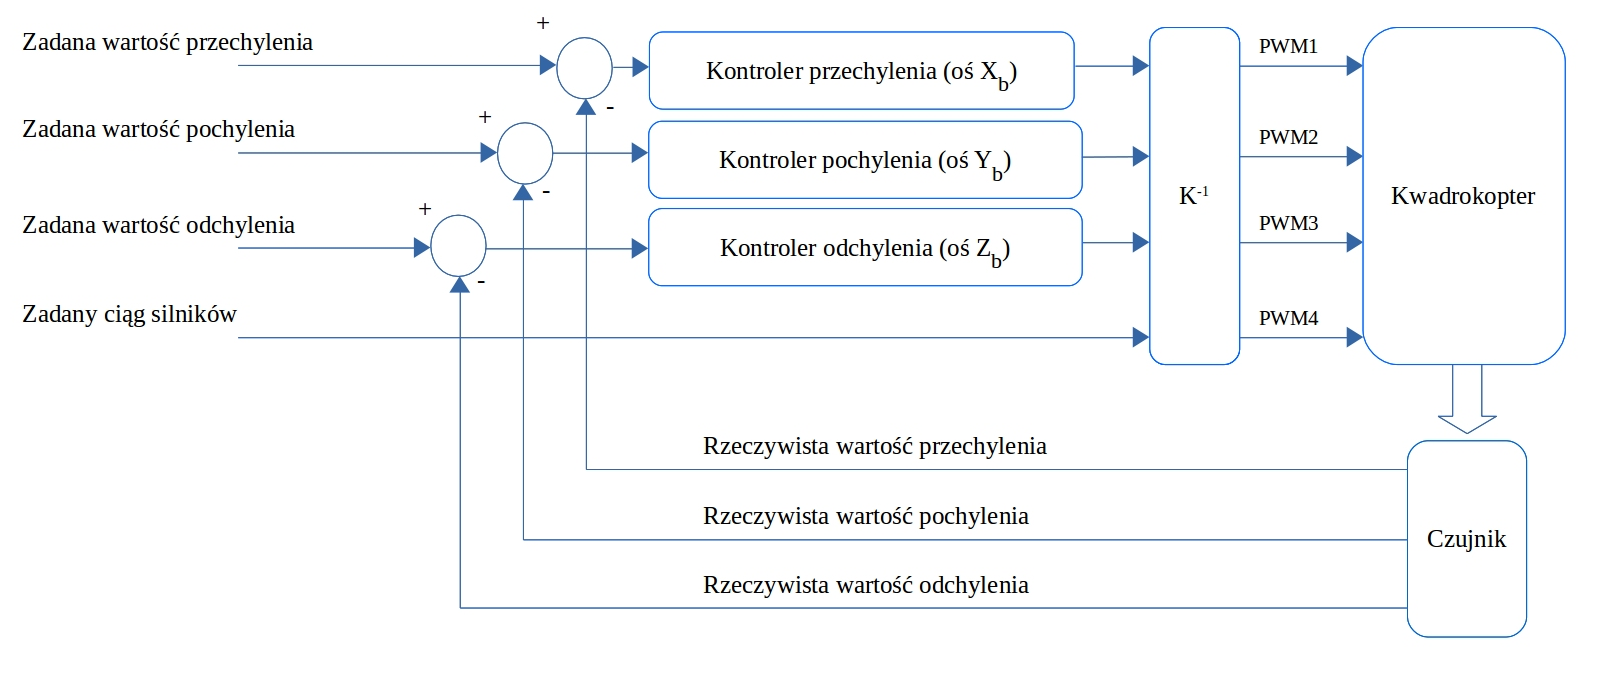
\includegraphics[width=1.1\textwidth]{Pictures/rate_controll_algorithm2.png}
		%\rule{35em}{0.5pt}
		\caption[Najprostszy algorytm kontroli lotu kwadrokoptera]{Najprostszy algorytm kontroli lotu kwadrokoptera}
	\label{fig:rate_controll_algorithm}
\end{figure}

Rysunek ~\ref{fig:rate_controll_algorithm} przedstawia strukturę omawianego algorytmu, zdolnego do kontroli prędkości obrotowej kwadrokoptera wokół każdej z trzech osi. Wartości zadane prędkości obrotowych wokół trzech osi układu współrzędnych transmitowane są drogą radiową, po czym trafiają na wejścia trzech regulatorów, odpowiedzialnych za utrzymanie stałych prędkości kątowych. Wartości wyjściowe z regulatorów wraz z wypadkową wartością ciągu wszystkich silników (również transmitowaną radiowo) konwertowane są następnie na wartości czterech sygnałów PWM, sterujących silnikami. Efektem sterowania silnikami jest pewnien określony obrót kwadrokoptera w trójwymiarowej przestrzeni, który jest z kolei mierzony za pomocą czujnika (na przykład trzyosiowego żyroskopu). Rzeczywiste wartości prędkości kątowych kwadrokoptera są następnie wykorzystywane przez regulatory w pętli sprzężenia zwrotnego, w celu wprowadzenia ewentualnej poprawki w wartościach sygnałów PWM. Algorytm nie precyzuje jaki rodzaj kontrolera ma być użyty, zatem najczęsciej używany jest regulator PID, głównie ze względu na prostotę implementacji oraz szeroki zasób materiałów dostępnych na jego temat~\cite{quadro9}.

Omawiany algorytm jest bardzo prosty w implementacji, dzięki czemu można go zastosować nawet w mikrokontrolerach, wyposażonych w niewielkie zasoby sprzętowe. Daje on bardzo dużą kontrolę nad kwadrokopterem - przy ustawieniu zadanej prędkości obrotowej na przykład wokół osi $X_b$ na wartość \SI{30}{\degree\per\second} kwadrokopter będzie się obracał z taką prędkością niezależnie od jego położenia względem ziemi. Pozwala to na wykonywanie rozmawitych akrobacji, jednakże wymaga od pilota dużej wprawy w sterowaniu maszyną, ze względu na konieczność ręcznej stabilizacji położenia kwadrokoptera względem ziemi. Dla przykładu, jeśli wychylimy drążek przechylenia, kwadrokopter w konfiguracji pokazanej na rysunku  ~\ref{fig:quadrotor_forces} otrzyma informację odnośnie prędkości obrotowej wokół osi $Y_b$ i zacznie poruszać się wzdłuż osi $X_e$. W momencie gdy użytkownik cofnie drążek wychylenia do pozycji spoczynkowej kwadrokopter przestanie obracać się  wokół osi $Y_b$, jednak ruch wzdłuż osi $X_e$ nie ustanie. Chcąc powrócić do stanu zawisu w powietrzu, użytkownik sam musi przesunąć drążek wychylenia w przeciwną stronę, tak aby kwadrokopter powrócił do pozycji poziomej. 

\section{Algorytm kontroli położenia kątowego}

Dla wielu uzytkowników brak automatycznej stabilizacji ruchu w płaszczyźnie poziomej może być uciążliwy, dlatego też warto zastanowić się co należy zrobić, aby zamiast kontroli nad prędkościami kątowymi wokół osi $X_b$ oraz $Y_b$ móc kontrolować kąt przechylenia ($\phi$) lub kąt wychylenia kwadrokoptera ($\theta$). Najprostszym rozwiązaniem będzie rozszerzenie algorytmu przedstawionego na rysunku ~\ref{fig:rate_controll_algorithm} tak, aby na wejściu zamiast prędkości kątowych wokół osi $X_b$ i $Y_b$ przyjmował docelowe wartości kątów przechylenia i odchylenia. Od razu w oczy rzuca się podstawowy problem: w poprzedniej wersji algorytmu, chcąc kontrolować prędkość kątową, wykorzystywano rzeczywistą wartość prędkości kątowej kwadrokoptera w pętli sprzężenia zwrotnego. Przy chęci kontrolowania kąta przechylenia lub wychylenia, rozszerzona wersja algorytmu musi wykorzystać w pętli sprzężenia zwrotnego informację o rzeczywistym kącie wychylenia lub przechylenia o jaki obrócił się kwadrokopter. Dlatego też aby omawiany algorytm miał prawo działać, należy zastanowić się, w jaki sposób można uzyskać wspomniane kąty.  

Obecnie dostępne czujniki, które można zamontować na prostym modelu kwadrokoptera, nie umożliwiają bezpośredniego pomiaru kątów przechylenia i wychylenia, dlatego też trzeba będzie sięgnąć do bardziej wyrafinowanych metod, bazujących na operacjach matematycznych dokonywanych na wynikach pomiarów z czujników takich jak:

\begin{itemize}
	\item Żyroskop
	\item Akcelerometr
\end{itemize} 

Wykorzystanie żyroskopu polega na całkowaniu jego pomiarów (prędkości kątowych) w czasie, tak aby uzyskać wartości kątów obrotu wokół odpowiednich osi. Rozwiązanie to ma jednak jedną wadę - sygnały wyjściowe obecnie produkowanych  żyroskopów zawsze obarczone są niewielkim błędem (zależnym od temperatury i zmiennym w czasie), który będąc całkowany razem z rzeczywistą wartością prędkości obrotowej doprowadziłby do znacznej różnicy między rzeczywistą wartością kąta obrotu a wartością wynikającą z policzonej całki~\cite{quadro9, filters1}. Sprawia to, że pomiar kąta obrotu dokonany za pomocą takiej metody nie jest miarodajny.

Wykorzystanie akcelerometru polega na odczytywaniu przyspieszeń liniowych wzdłuż każdej z osi kwadrokoptera, a następnie na przekształceniu ich za pomocą funkcji trygonometrycznych na wartości kątów przechylenia i wychylenia zgodnie z poniższymi wzorami~\cite{mems5}:

\begin{equation}
	\phi = \arctan(\frac{a_y}{\sqrt{a{_z}^2 + a{_x}^2}})
\end{equation}

\begin{equation}
	\theta = \arctan(\frac{a_x}{\sqrt{a{_z}^2 + a{_y}^2}})
\end{equation}

gdzie wartości $a_x$, $a_y$, $a_z$ są wartościami przyspieszeń liniowych mierzonych wzdłuż osi odpowiednio $X_b$, $Y_b$, $Z_b$.

Podane rozwiązanie nie jest jednak idealne. Zadziałanie na kwadrokopter zewnętrznej siły (np. pudmuch wiatru) nadającej mu dodatkową wartosć przyspieszenia może powodować błędną interpretację odbieranych pomiarów przez algorytm kontroli lotu. Co więcej, akcelerometr jest czujnikiem bardzo wrażliwym na wibracje, które będą powodować błąd między rzeczywistym kątem pochylenia lub przechylenia a kątem obliczonym na podstawie pomiarów.

Reasumując mamy dwie metody estymacji kąta pochylenia i przechylenia, obarczone następującymi niedoskonałościami:

\begin{itemize}
	\item Całkowanie prędkości kątowej w czasie:
		\begin{itemize}
			\item wartość wyjściowa obarczona błędem, który całkowany w czasie powoduje coraz większą odchyłkę wartości rzeczywistej kąta od wartości obliczonej.
		\end{itemize}
	\item Wykorzystanie wskazań z akcelerometru i funkcji trygonometrycznych:
		\begin{itemize}
			\item zewnętrzne siły mogą powodować błędną interpretację pomiarów przez algorytm kontroli lotu,
			\item duża czułość akcelerometru na wibracje powoduje niedokładność estymacji kąta.
		\end{itemize}
\end{itemize}

W świetle niedoskonałości każdej z dwóch wspomnianych metod, rozwiązaniem problemu będzie połączenie wartości pomiarów obu czujników i wykorzystanie odpowiedniej funkcji fuzji danych z sensorów (ang. sensor fusion function), umożliwiającej estymację położenia kwadrokoptera w przestrzeni~\cite{filters1}.

Wśród wielu znanych funkcji, które mogą zostać użyte do obliczania położenia kwadrokoptera w przestrzeni, wyróżnić można dwie najbardziej popularne~\cite{filters1, filters2, filters3}:
\begin{itemize}
	\item Filtr Kalmana
	\item Filtry komplementarne
\end{itemize}

Filtr Kalmana, jest to algorytm rekurencyjny, który służy do określenia stanu badanego układu dynamicznego na podstawie jego modelu matematycznego (np. równań ruchu) oraz serii pomiarów wejścia i wyjścia tego układu. Algorytm ten, składa się z dwóch kroków:

\begin{itemize}
	\item Faza predykcji - służy do określenia przewidywanego następnego stanu procesu, w oparciu o znajomość poprzedniego stanu procesu.
	\item Faza korekcji - na podstawie rzeczywistych wartości pomiarów dokonuje się aktualizacji estymaty stanu procesu, a także określa się jak bardzo wartość estymaty z kroku poprzedniego odbiegała od wartości rzeczywistej
\end{itemize} 

Filtr Kalmana jest bardzo popularny w zastosowaniach łączenia danych z sensorów w celu określenia położenia statków powietrznych, jednakże jego złożoność obliczeniowa dyskfalifikuje go do zastosowań w małych kontrolerach lotu (np. opartych o architekturę AVR).

\begin{figure}[H]
	\centering
	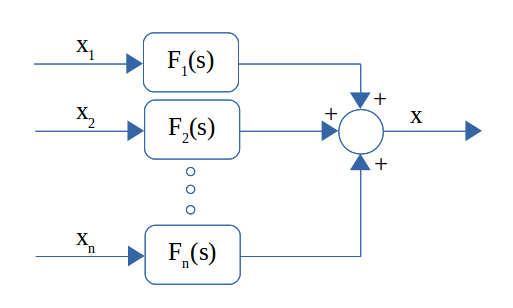
\includegraphics[width=0.7\textwidth]{Pictures/complementary_filter_general.png}
		%\rule{35em}{0.5pt}
		\caption[Struktura filtru komplementarnego]{Struktura filtru komplementarnego}
	\label{fig:complementary_filter_general}
\end{figure}

Rysunek ~\ref{fig:complementary_filter_general} przedstawia strukturę filtru komplementarnego. Idea jego działania polega na łączeniu danych z różnych czujników, z których każdy narażony jest na zakłócenia o różnych częstotliwościach, usuwanie zakłóceń za pomocą odpowiednich filtrów (dolnoprzepustowych, górnoprzepustowych lub pasmowoprzepustowych) a następnie łączeniu przefiltrowanych sygnałów w wartość ostateczną. Filtr komplementarny powinien spełniać następujący warunek:

\begin{equation}
	\sum_{i=1}^{n}F_{i}(s) = 1
\end{equation}

Rzutując tę ideę na model kwadrokoptera, filtr taki może zostać użyty do łączenia danych z żyroskopu oraz akcelerometru. Wartości z żyroskopu dryfują w czasie, a zatem obarczone są błędem o niskiej częstotliwości, dlatego też do ich filtrowania użyty zostanie filtr górnoprzepustowy. Wartości z akcelerometrów zakłocone są drganiami generowanymi przez silniki oraz ruchami kwadrokoptera, a zatem są to zakłócenia o wysokicz częstotliwościach i do ich zniwelowania użyty zostanie filtr dolnoprzepustowy. Następnie przefiltrowane wartości po dokonaniu odpowiednich operacji matematycznych, mogą zostać wykorzystane do obliczenia kąta przechylenia i pochylenia kwadrokoptera.

Mając wiedzę na temat najbardziej popularnych funkcji fuzji danych z czujników, możemy powrócić do omawiania algorytmu kontroli położenia kwadrokoptera w przestrzeni, którego struktura została przedstawiona na rysunku~\ref{fig:angle_control_algorithm}.

\begin{figure}[H]
	\centering
	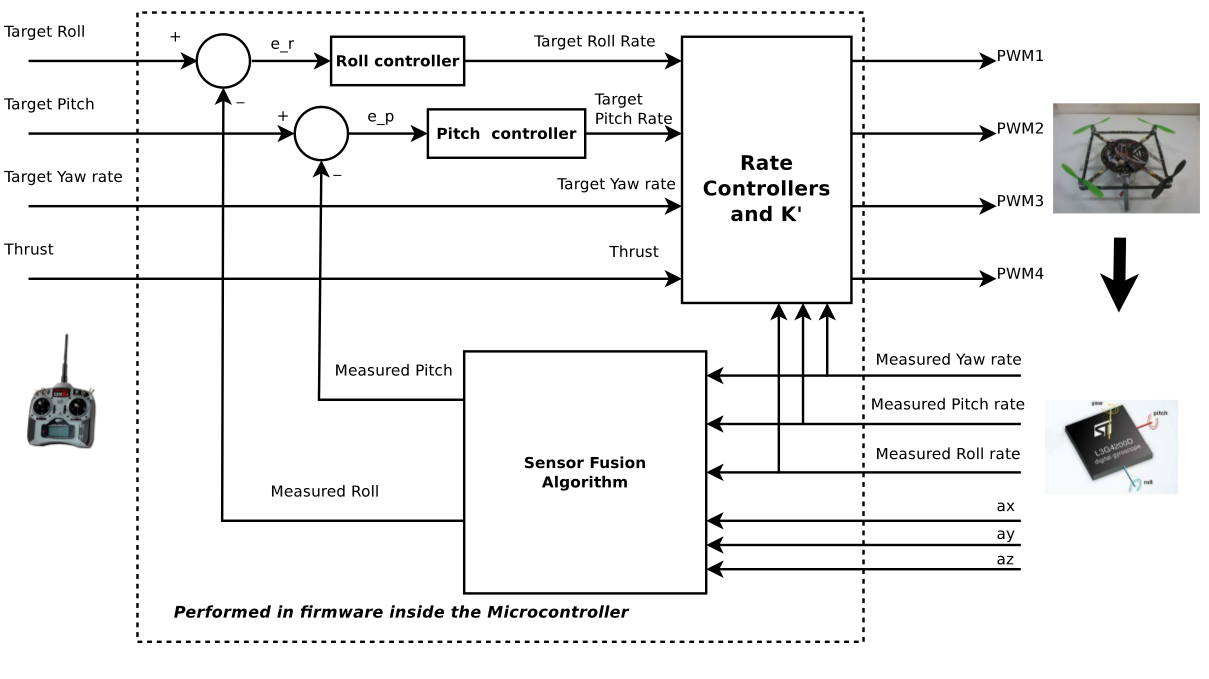
\includegraphics[width=1.0\textwidth]{Pictures/angle_control_algorithm.png}
		%\rule{35em}{0.5pt}
		\caption[Algorytm kontroli położenia kwadrokoptera]{Algorytm kontroli położenia kwadrokoptera~\cite{quadro9}}
	\label{fig:angle_control_algorithm}
\end{figure}

Jak widać w tej wersji algorytmu drogą radiową przesyłane są (oprócz wartości wypadkowego ciągu oraz zadanej prędkości kątowej wokół osi $Z_b$) docelowe wartości kątów przechylenia i pochylenia, jakie ma osiągnąć kwadrokopter. Wartości te trafiają razem z rzeczywistymi kątami przechylenia i pochylenia, o jakie obecnie obrócił się kwadrokopter na wejścia dwóch regulatorów, odpowiedzialnych za utrzymanie zadanego położenia kątowego w płaszczyźnie poziomej. Sygnały wyjściowe z wspomnianych dwóch regulatorów są prędkościami kątowymi wokół osi $X_b$ i $Y_b$, jakie kwadrokopter powinien uzyskać w danej chwili, aby dążyć do docelowej orientacji w przestrzeni. Trafiają one wraz z wartością wypadkowego ciągu silników oraz zadaną prędkością kątową wokół osi $Z_b$ do bloku kontrolującego prędkości kątowe wokół wszystkich osi układu odniesienia, czyli do algorytmu omawianego w poprzednim podrozdziale. 

Algorytm w takiej postaci będzie zdolny do automatycznego wypoziomowania kwadrokoptera po puszczeniu przez pilota drążka przechylenia/wychylenia. Jest on bardziej złożony obliczeniowo  oraz daje mniejszą kontrolę nad kwadrokopterem w porównaniu do algorytmu omawianego w poprzednim podrozdziale, jednakże ze względu na wygodę użytkowania jest częściej stosowany w amatorskich konstrukcjach.
 

%----------------------------------------------------------------------------------------
%	SECTION 2
%----------------------------------------------------------------------------------------

